% !TeX program = xelatex
% !TeX encoding = UTF-8 Unicode
% !BIB program = biber

% essa classe aceita as seguintes opções:
% abnd ou ieee pra estilo de citaçõ
% english ou french pra língua dos slides (não passar nada é português)
% minted pra usar o pacote minted (configurado para python e C)
% final para imprimir todas as folhas requeridas pela versão final. O arquivo
% ficha.pdf, provido pela coordenação, deverá estar presente.
\documentclass[minted]{tcc}

% Essa classe usa o biblatex com backend biber ao invés do bibtex.
\addbibresource{bibliothek.bib}

% Controla o texto das captions das figuras. Neste caso, centraliza.
\captionsetup{justification=centering}

\title{Template de TCC}

% Todo comando \add trabalha com uma lista e todo comando \set trabalha com um
% único elemento, ou seja, pode haver apenas um \setorientador mas vários
% \addauthor. Todo comando \add e \set tem um \get correspondente (por exemplo,
% \getauthors, \getsubject). Esses comandos são definidos na classe
% relatorio.cls. No caso dos \set, os \get são implicitos, e não você não vai
% encontrá-los na classe.

\addauthor{Álan Crístoffer e Sousa}{acristoffers@ieee.com}

\setorientador{Prof.\ Dr.\ Valter Júnior de Souza Leite}
\addcoorientador{Prof.\ Dr.\ Ignacio Rubio Scola}

\setcoordenador{Prof.\ Dr.\ Lúcio Flávio Santos Patrício}
\addmembrobanca{Prof.\ Me.\ Alberto Pena Lara}
\addmembrobanca{Prof.\ Me.\ Adriano Nogueira Drumond Lopes}

\seteixodeformacao{Modelagem e Controle de Processos}

\setlocal{Divinópolis}
\setano{2018}
\setmes{Dezembro}

\setdedicatoria{A minha família, que sempre me apoiou nessa caminhada.}
\setfrase{Não há nada como um sonho para criar o futuro.}
\setfraseautor{Victor Hugo}
\setagradecimentos{aos meus pais por todo o apoio e confiança em mim depositados;\\[2mm]
  ao Prof.\ Valter por toda a paciência e empenho nesses 2 anos de orientação;\\[2mm]
  ao Prof.\ Ignacio pelas conversas e esclarecimentos;\\[2mm]
  aos colegas de trabalho mais próximos: Nelson Figueredo, Ângelo Eugênio,
  Mariella Maia, Michelle Faria, Anderson Bento, Mário Cipriano, Bernardo Amim,
  Luis Gustavo e Rafael Silveira a convivência descontraída e as trocas de
  experiências;\\[2mm]
  aos demais colegas do Grupo de Modelagem e Controle de Sistemas Mecatrônicos a
  ótima convivência;\\[2mm]
  a todos que de alguma forma contribuíram com o meu progresso.}

\preamble{}

% !TeX root = document.tex
% !TeX encoding = UTF-8 Unicode

% probably a good idea for the nomenclature entries:
\acsetup{list/template=longtable,make-links=true}

\ExplSyntaxOn
\cs_set_protected:Npn \acro_activate_hyperref_support:
  {
    \bool_if:nT { \l__acro_hyperref_loaded_bool }
      {
        \sys_if_engine_xetex:TF
          {
            \cs_set:Npn \acro_hyper_link:nn ##1##2
             { \hyperlink {##1} { \XeTeXLinkBox{##2} } } 
          }
          { \cs_set_eq:NN \acro_hyper_link:nn \hyperlink }
        \cs_set:Npn \acro_hyper_target:nn ##1##2
          { \raisebox { 3ex } [ 0pt ] { \hypertarget {##1} { } } ##2 }
      }
  }
\ExplSyntaxOff

\DeclareAcronym{LPV}{
    short = LPV,
    long  = {Variação linear de parâmetros, do inglês \textit{Linear Parameter Varying}},
    tag = abbrev
}

\DeclareAcronym{MPC}{
    short = MPC,
    long  = {Controle preditivo por modelo, do inglês \textit{Model Predictive Control}},
    tag = abbrev
}

\DeclareAcronym{DMPC}{
    short = DMPC,
    long  = {Controle preditivo por modelo discreto, do inglês \textit{Discrete Model Predictive Control}},
    tag = abbrev
}

\DeclareAcronym{SPD}{
    short = SPD,
    long  = Sistema a Parâmetros Distribuídos,
    tag = abbrev
}

\DeclareAcronym{SPC}{
    short = SPC,
    long  = Sistema a Parâmetros Concentrados,
    tag = abbrev
}

\DeclareAcronym{DMC}{
    short = DMC,
    long  = {Controle Dinâmico por Matriz, do inglês \textit{Dynamic Matrix Control}},
    tag = abbrev
}

\DeclareAcronym{IMC}{
    short = IMC,
    long  = {Controle por Modelo Interno, do inglês \textit{Internal Model Control}},
    tag = abbrev
}

\DeclareAcronym{EDP}{
    short = EDP,
    long  = Equação Diferencial Parcial,
    tag = abbrev
}

\DeclareAcronym{ARMAX}{
    short = ARMAX,
    long  = {Modelo autoregressivo de média variável com entradas exógenas, do inglês \textit{Autoregressive–moving-average with exogenous inputs model}},
    tag = abbrev
}

\DeclareAcronym{AT}{
    short = \(A'\),
    long  = Transposta de uma matriz,
    sort  = A',
    tag = nomencl
}


\begin{document}
\maketitle{}
% !TeX root = document.tex
% !TeX encoding = UTF-8 Unicode

\IEEEtitleabstractindextext{%
\begin{abstract}
  O controle discreto no tempo se aproxima mais da realidade atual, onde o
  controle é feito de forma digital. As leis de controle implementadas
  utilizando sistemas discretos podem ser escritas com funções simples,
  normalmente de soma e multiplicação de termos, que são fáceis de interpretar
  e, principalmente, de implementar em um sistema digital. Por tratar o sistema
  como digital, ele leva em conta problemas da natureza desses sistemas, como o
  tempo de amostragem, normalmente apenas ignorados em implementações contínuas
  nesses sistemas. Este trabalho visa a implementação de dois controladores
  digitais em um sistema massa-mola em plano inclinado, visando demonstrar a
  síntese e implementação de tais controladores, e a análise desses sistemas.
\end{abstract}

\begin{IEEEkeywords}
  controle digital, jury, espaço de estados
\end{IEEEkeywords}
}

\toc{}

% !TeX root = document.tex
% !TeX encoding = UTF-8 Unicode

\chapter{Floats}
\section{Figuras}

Adicione figuras com o ambiente \texttt{figure} e referencie com \texttt{ref}. A
palavra antes da referência sempre tem inicial maíuscula: Figura~\ref{fig:smm1}.
O til entre Figura e o comando \texttt{ref} é um espaço que não pode ser
quebrado.

\begin{figure}[ht!] % ht! é o posicionamento da figura.
  \centering % centraliza a figura no ambiente figure
  % Ajuste o tamanho da figura usando a porcentagem em frente à \linewidth.
  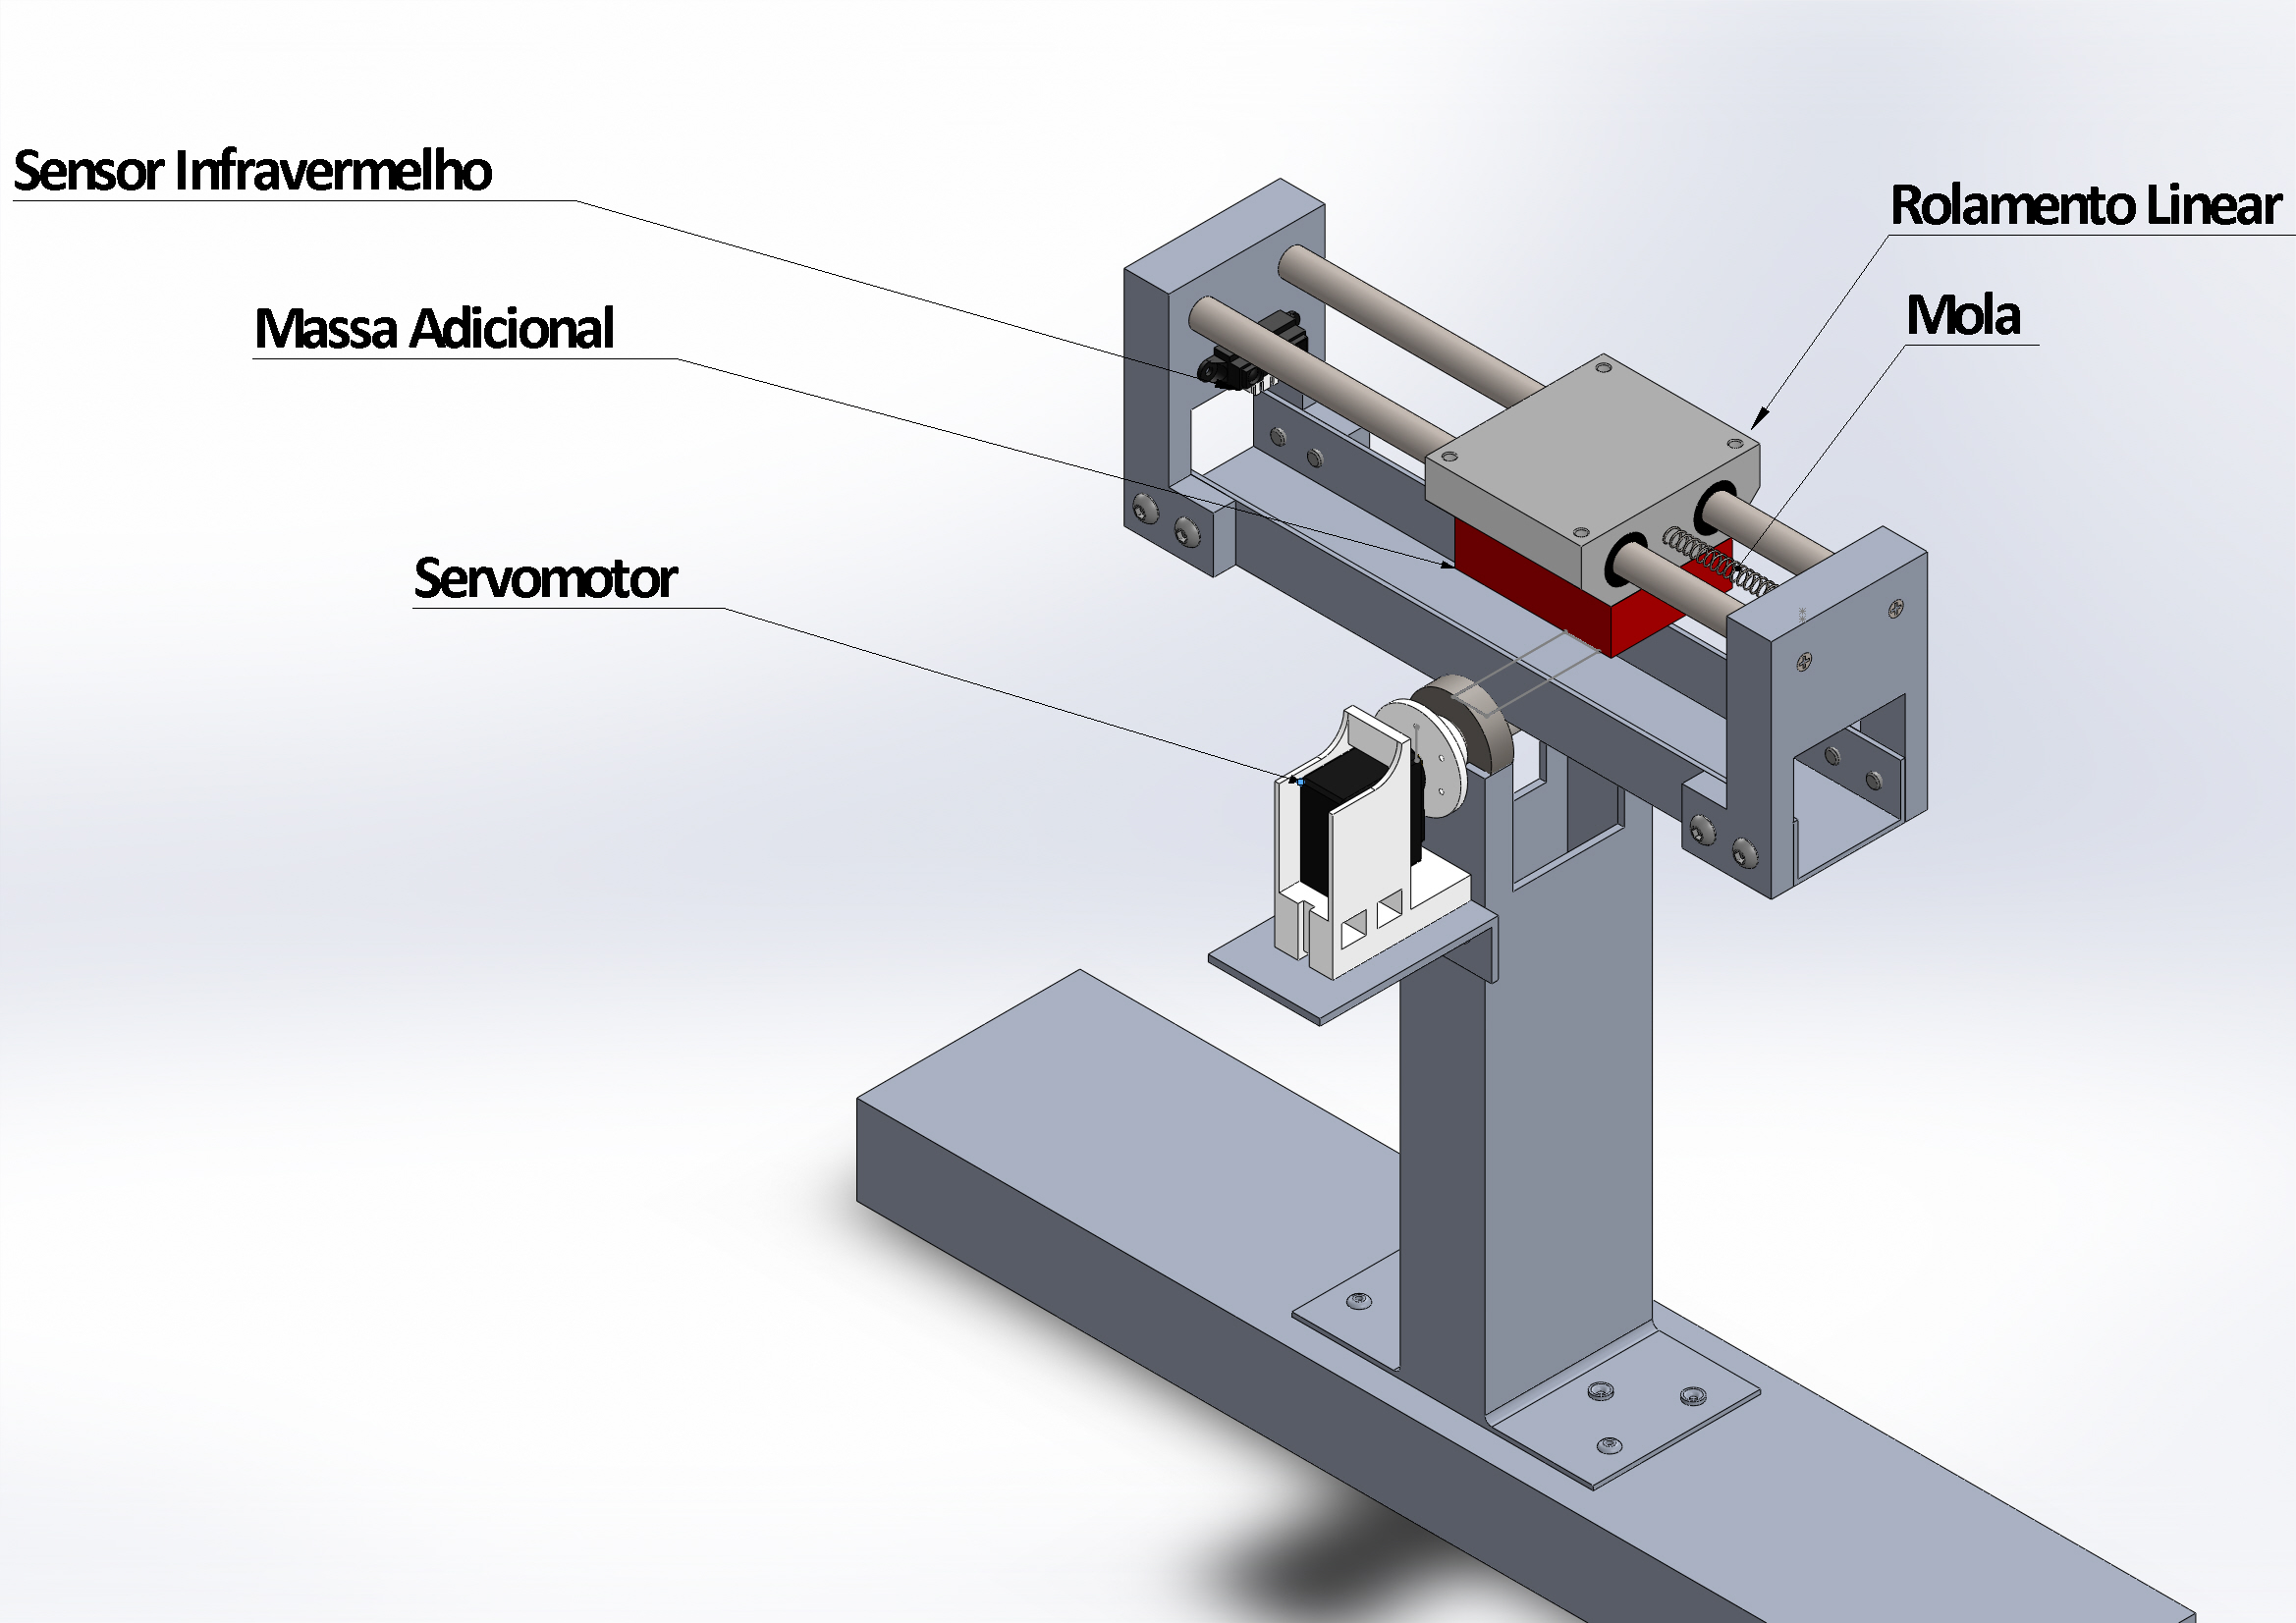
\includegraphics[width=0.9\linewidth]{planta}
  % texto que aparece abaixo da figura. O % no fim da linha anula a quebra de
  % linha, o que faz com que o \label fique junto com o caption, evitando erro
  % de offset quando o usuário clicar em um reflink no PDF. Eu uso inícios
  % padões em toda label: fig, eq, tbl, sec, subsec, chp... e recomendo que você
  % faça o mesmo.
  \caption{Sistema Massa-Mola}%
  \label{fig:smm1}
\end{figure}

Na Figura~\ref{fig:smm2} temos um exemplo de subfiguras.

\begin{figure}[ht!]
  \centering
  \subbottom[One]{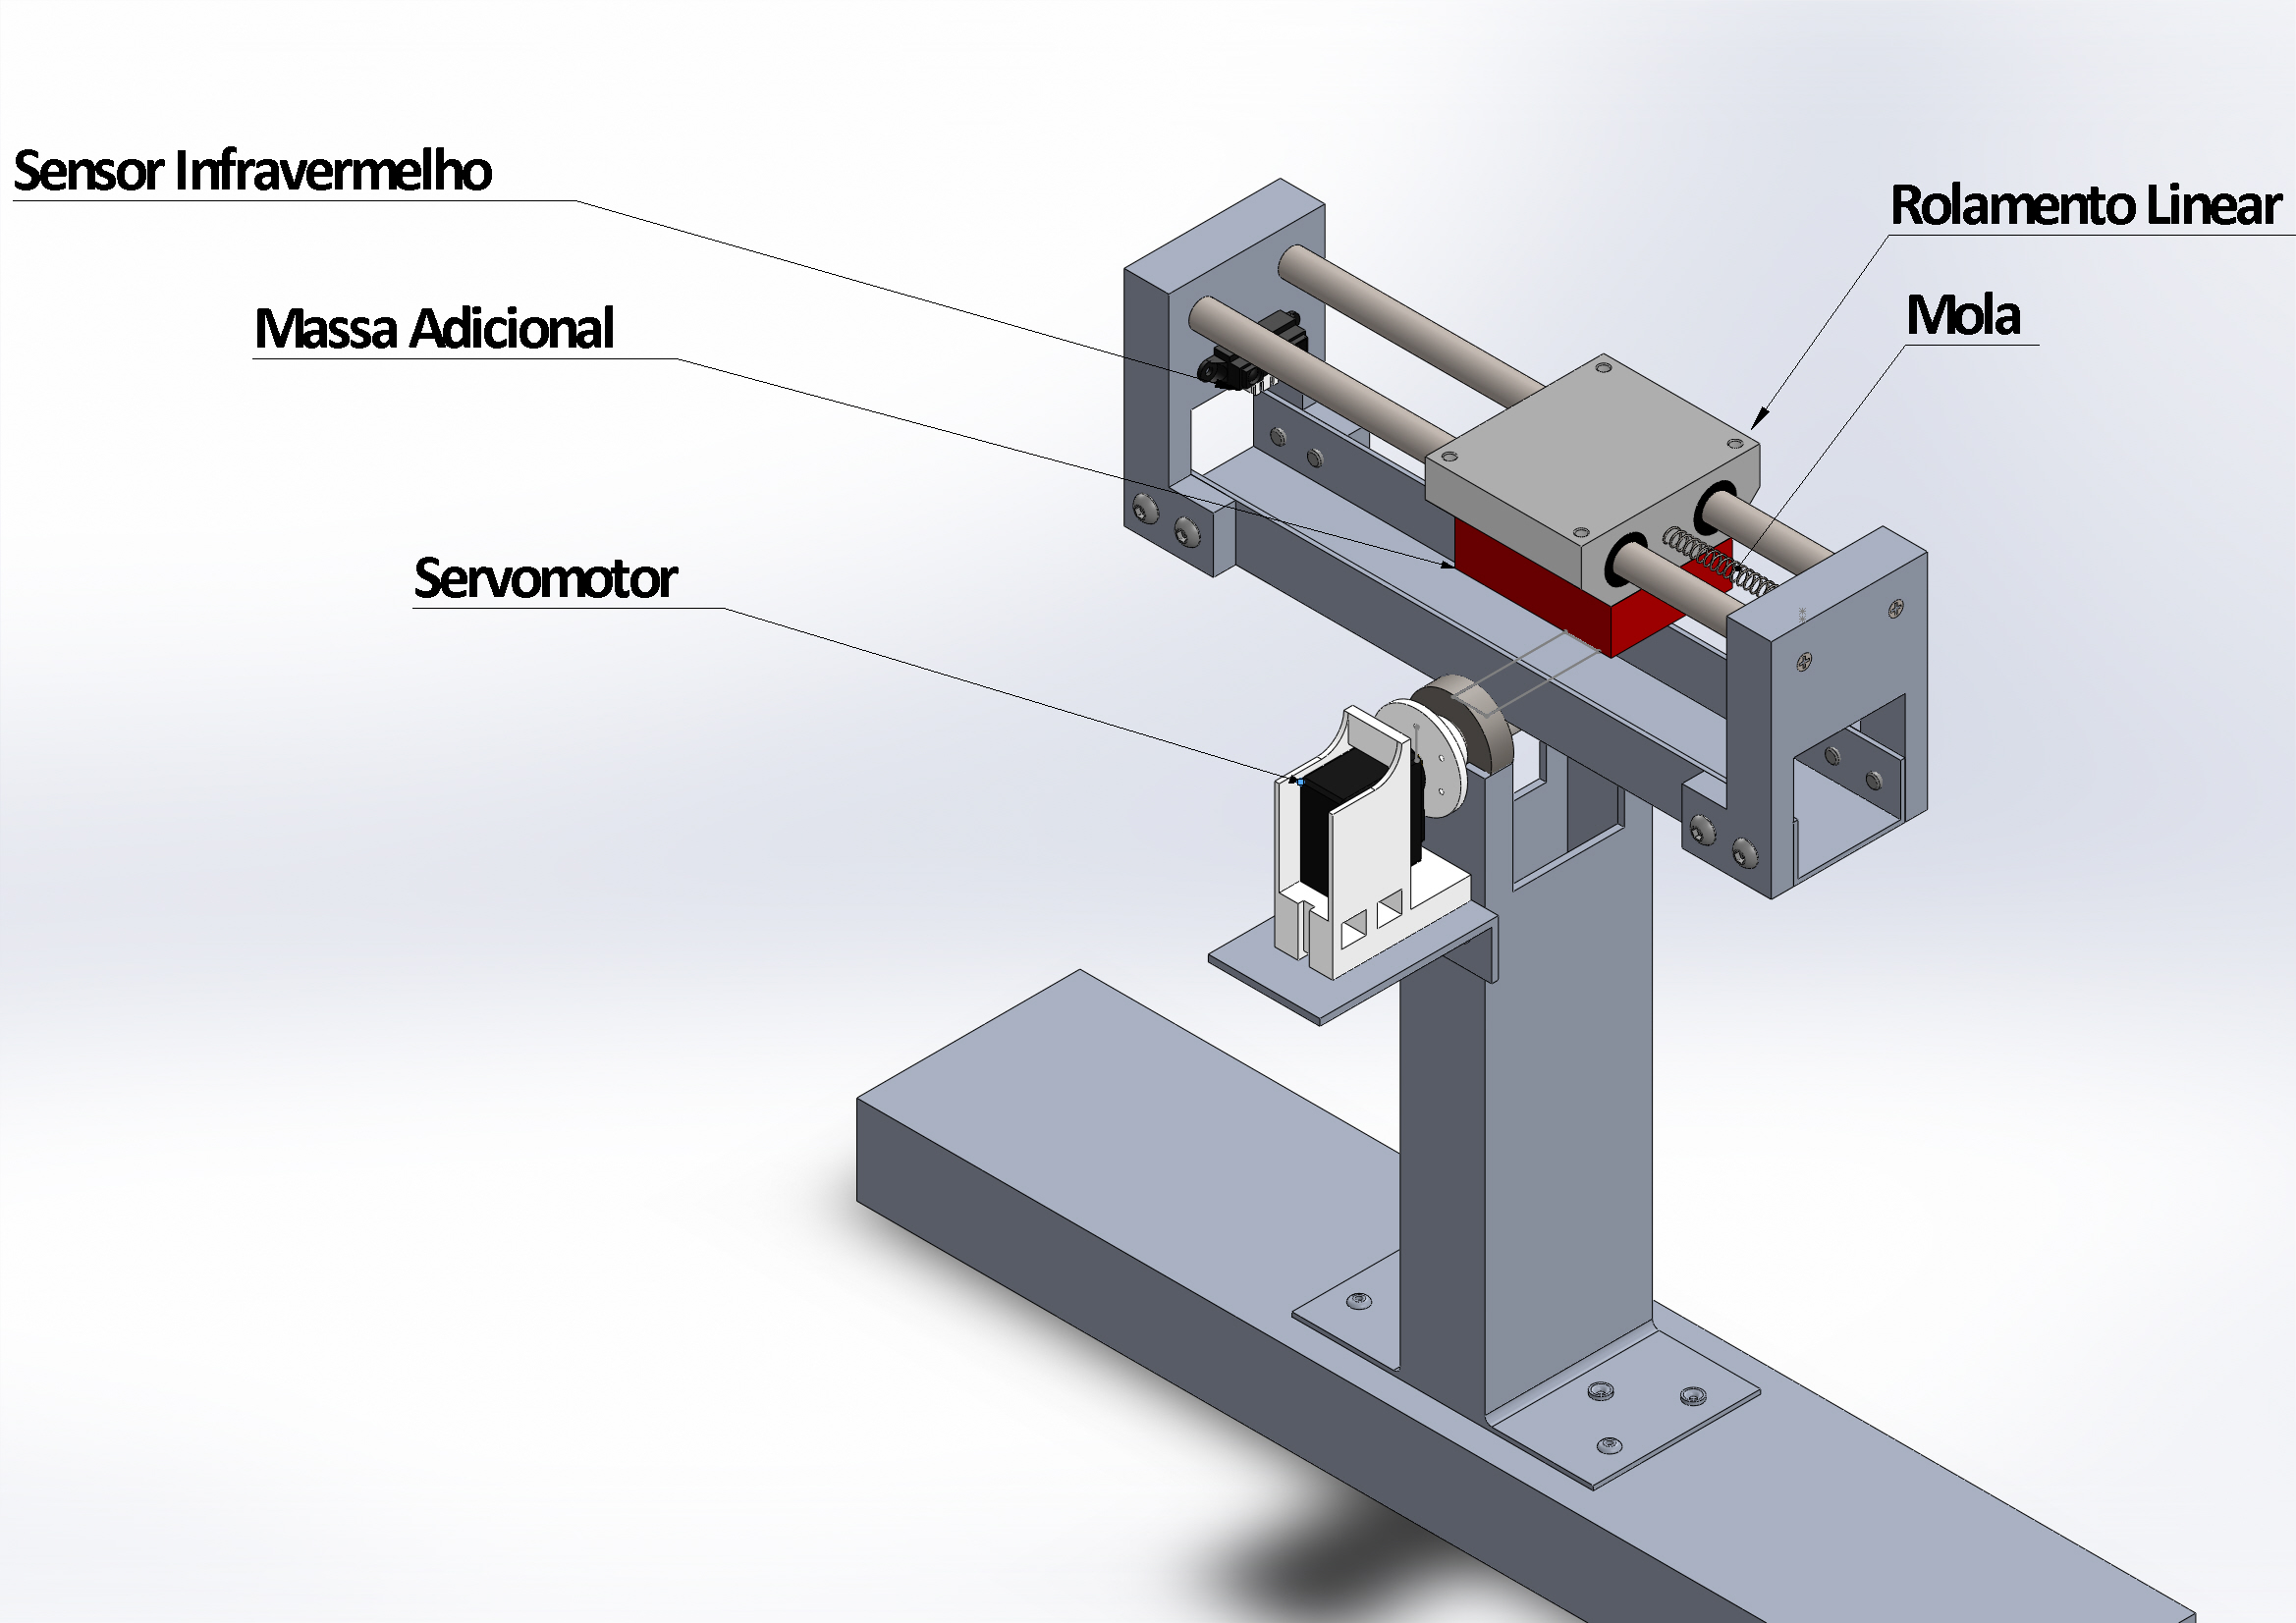
\includegraphics[width=0.4\linewidth]{planta}}\qquad
  \subbottom[Two]{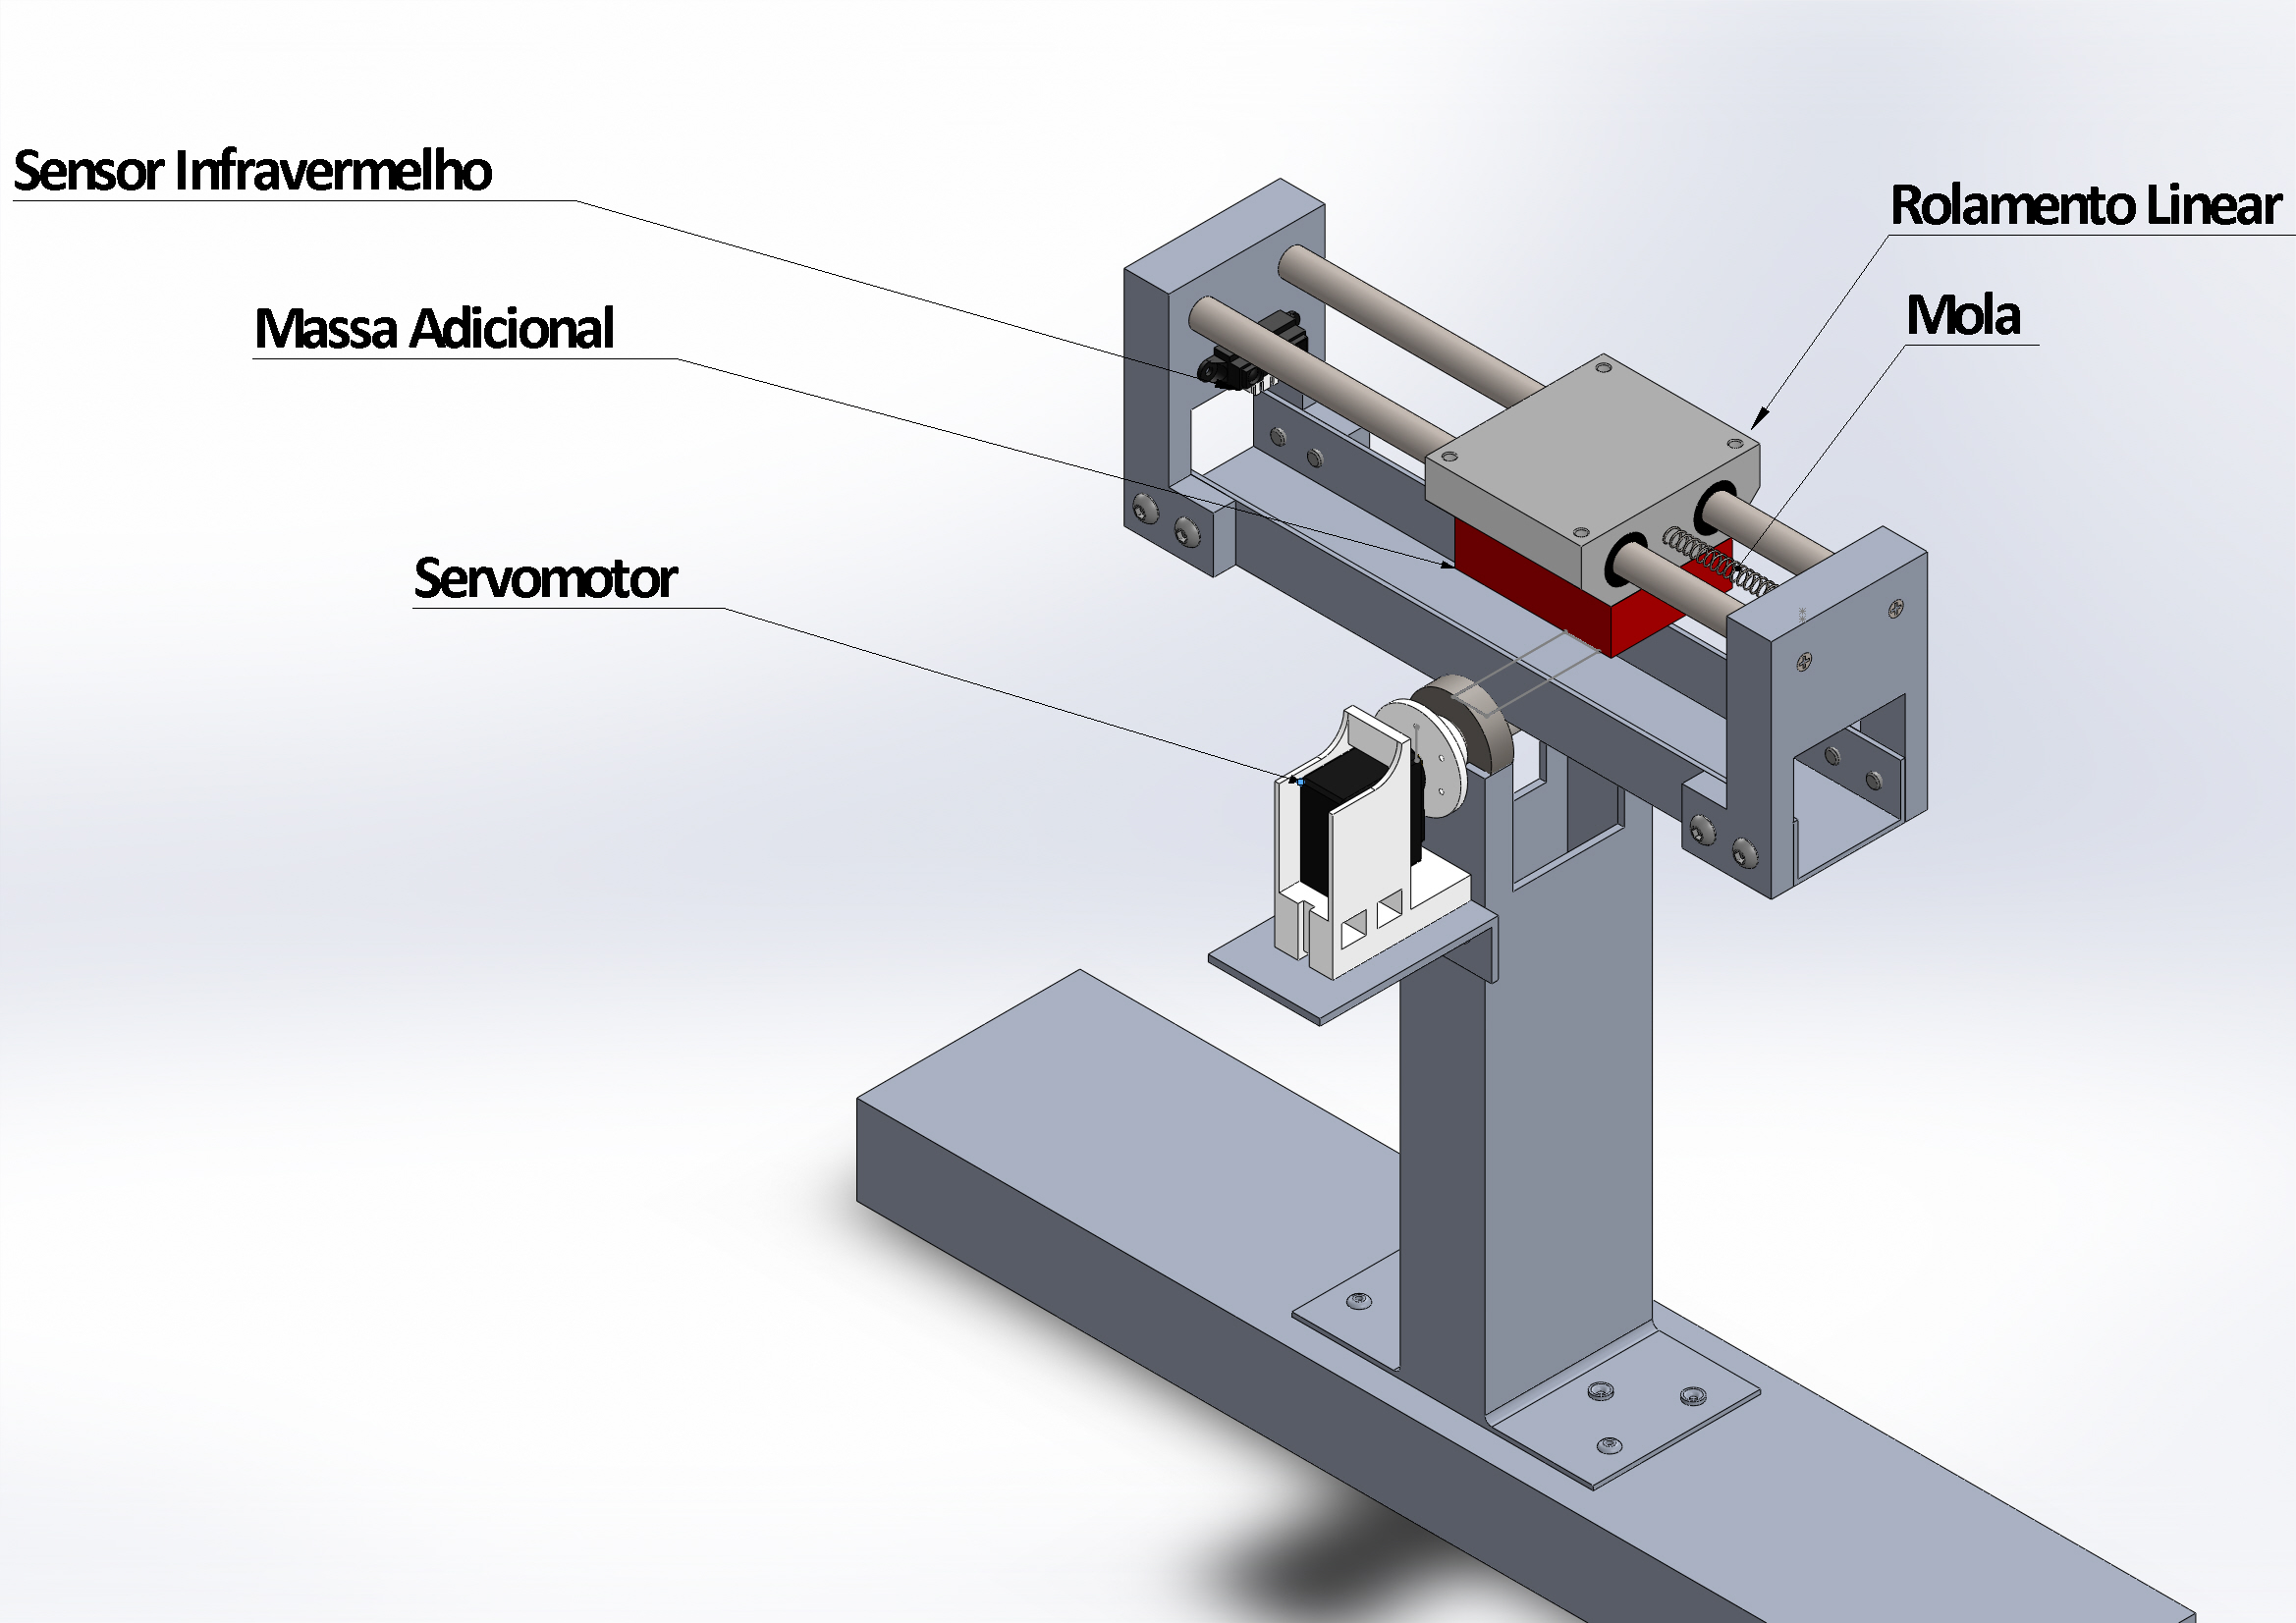
\includegraphics[width=0.4\linewidth]{planta}}
  \caption{Dois sistemas massa-mola.}%
  \label{fig:smm2}
\end{figure}

\FloatBarrier % impede que as figuras já definidas passem para a próxima seção.
% O Latex sempre tenta posicionar os floats (figura/tabelas) e o texto de forma
% eficiente quanto ao espaço, então em várias situações ele vai mandar a figura
% pra próxima página ou atravessar pra próxima seção. Se isso não é desejado,
% basta usar o \FloatBarrier que todos os floats declarados que ainda não foram
% posicionados serão posicionados nesse ponto. Se não entendeu, remova e veja a
% diferença no posicionamento das figuras e tabela em relação ao texto.

\section{Tabela}

A Tabela~\ref{tbl:exemplo} mostra como fazer uma tabela com ou sem linhas.

% Eu uso https://www.tablesgenerator.com pra gerar a tabela, e depois edito.
\begin{table}[ht!]
  \centering
  % Você deve fornecer um alinhamento para cada coluna. O símbolo | entre as
  % colunas indica que uma linha será desenhada.
  \begin{tabular}{l|cccc}
    \toprule
    Professor & Mecânica       & Eletrônica     & Controle       & Programação    \\ \midrule
    Lúcio     & \(\checkmark\) &                &                &                \\
    Valter    &                &                & \(\checkmark\) &                \\
    Thiago    &                &                &                & \(\checkmark\) \\
    Marlon    &                & \(\checkmark\) &                &                \\
    \bottomrule
  \end{tabular}
  \caption{Eixo de professores.}%
  \label{tbl:exemplo}
\end{table}
% Este exemplo mostra como usar top/mid/bottom rules e linhas verticais. No
% entanto, o povo do latex não recomenda usar isso dizendo que fica feio. No
% fim do dia o documento é seu, use ou não se quiser.

% !TeX root = document.tex
% !TeX encoding = UTF-8 Unicode

\chapter{Listas}
\section{Lista Simples}

Lista com números:

\begin{enumerate}
  \item One
  \item Two
  \item Three
\end{enumerate}

Lista sem números:

\begin{itemize}
  \item One
  \item Two
  \item Three
\end{itemize}

\section{Lista Com Numeração Diferente}

Lista com números romanos:

\begin{enumerate}[I]
  \item One
  \item Two
        \begin{enumerate}[i]
          \item One
          \item Two
          \item Three
        \end{enumerate}
  \item Three
\end{enumerate}

\begin{enumerate}[(I)]
  \item One
  \item Two
        \begin{enumerate}[(i)]
          \item One
          \item Two
          \item Three
        \end{enumerate}
  \item Three
\end{enumerate}%

Lista com letras:

\begin{enumerate}[A]
  \item One
  \item Two
        \begin{enumerate}[a]
          \item One
          \item Two
          \item Three
        \end{enumerate}
  \item Three
\end{enumerate}

\begin{enumerate}[(A)]
  \item One
  \item Two
        \begin{enumerate}[(a)]
          \item One
          \item Two
          \item Three
        \end{enumerate}
  \item Three
\end{enumerate}%

\section{Lista Não Numerada}

Lista de descrição:

\begin{description}
  \item[PID] Predictive-Integral-Derivative
  \item[ABS] Absolute Bull Shit
  \item[IoT] Internet of Things
\end{description}

% !TeX root = document.tex
% !TeX encoding = UTF-8 Unicode

\chapter{Equações}
\section{Numeradas}

Equation:
\begin{equation}
  \dot{x} = Ax+Bu
\end{equation}

Align:
\begin{align}
  \dot{x} & = Ax+Bu \\
  y       & =Cx+Du
\end{align}

Equation+Aligned:
\begin{equation}
  \begin{aligned}
    \dot{x} & = Ax+Bu \\
    y       & =Cx+Du
  \end{aligned}
\end{equation}

\section{Não Numeradas}

Equation:
\begin{equation*}
  \dot{x} = Ax+Bu
\end{equation*}

Align:
\begin{align*}
  \dot{x} & = Ax+Bu \\
  y       & =Cx+Du
\end{align*}

Equation+Aligned:
\begin{equation*}
  \begin{aligned}
    \dot{x} & = Ax+Bu \\
    y       & =Cx+Du
  \end{aligned}
\end{equation*}

Align com epenas alguns items enumerados:
\begin{align}
  \dot{x} & = Ax+Bu           \\
  y       & = Cx+Du           \\
  c       & = Ex+Fu \nonumber % remove a numeração de uma equação
\end{align}

% !TeX root = document.tex
% !TeX encoding = UTF-8 Unicode

\chapter{Citações}
\section{Citações}

Para referenciar, há basicamente duas formas: \texttt{parencite} e
\texttt{textcite}. Eles são os equivalentes do biblatex aos comandos
\texttt{citep} e \texttt{citet} do bibtex. O primeiro serve para citar no fim do
parágrafo:

\begin{quote}
  Há quem diga que a lua é um queijo~\parencite{book:ogata}.
\end{quote}

O segundo para citar quando o nome do autor faz parte do texto:

\begin{quote}
  Segundo~\textcite{book:ogata}, a lua é um queijo.
\end{quote}

% !TeX root = document.tex
% !TeX encoding = UTF-8 Unicode

\chapter{Códigos}
\section{Códigos}

O pacote \texttt{minted} oferece um ambiente para apresentação de código com
\textit{syntax highlight}.

Python 3:

\begin{python3code}
#!/usr/bin/env python3


def fib(n):
    a = b = 1
    while n > 1:
        a, b, n = b, a + b, n - 1
    return b

import sys

if len(sys.argv) > 1:
    print(fib(int(sys.argv[1])))
else:
    print("This application finds the n'th fibonacci number.\nType the desired value for n:")
    print(fib(int(input())))
\end{python3code}
\captionof{listing}{Código Python3}%
\label{code:python-code}

C:

\begin{ccode}
#include <stdint.h>
#include <stdlib.h>

extern "C" {
    uint64_t fib(uint64_t n)
    {
        uint64_t a = 1;
        uint64_t b = 1;
        uint64_t c = 1;

        while (n-- > 2) {
            c = a + b;
            a = b;
            b = c;
        }

        return b;
    }
}
\end{ccode}
\captionof{listing}{Código C}%
\label{code:c-code}


\nocite{*} % Marca todas as referências dos arquivos bib como usadas. Todas
% irão aparecer no capítulo Referências.
\printbibliography{}
\end{document}
